% style setup
% -----------------------------------------------------------------------
\documentclass[10pt,landscape]{article}
\usepackage{amssymb,amsmath,amsthm,amsfonts}
\usepackage{amsmath}
\usepackage{amssymb}
\usepackage{multicol,multirow}
\usepackage[utf8]{inputenc}
\usepackage{calc}
\usepackage{ifthen}
\usepackage[landscape]{geometry}
\usepackage[colorlinks=true,citecolor=blue,linkcolor=blue]{hyperref}
\usepackage{graphicx}
\graphicspath{ {./images/} }

\ifthenelse{\lengthtest { \paperwidth = 11in}}
    { \geometry{top=.5in,left=.5in,right=.5in,bottom=.5in} }
	{\ifthenelse{ \lengthtest{ \paperwidth = 297mm}}
		{\geometry{top=1cm,left=1cm,right=1cm,bottom=1cm} }
		{\geometry{top=1cm,left=1cm,right=1cm,bottom=1cm} }
	}
\pagestyle{empty}
\makeatletter
\renewcommand{\section}{\@startsection{section}{1}{0mm}%
                                {-1ex plus -.5ex minus -.2ex}%
                                {0.5ex plus .2ex}%x
                                {\normalfont\large\bfseries}}
\renewcommand{\subsection}{\@startsection{subsection}{2}{0mm}%
                                {-1explus -.5ex minus -.2ex}%
                                {0.5ex plus .2ex}%
                                {\normalfont\normalsize\bfseries}}
\renewcommand{\subsubsection}{\@startsection{subsubsection}{3}{0mm}%
                                {-1ex plus -.5ex minus -.2ex}%
                                {1ex plus .2ex}%
                                {\normalfont\small\bfseries}}
\makeatother
\setcounter{secnumdepth}{0}
\setlength{\parindent}{0pt}
\setlength{\parskip}{0pt plus 0.5ex}
% -----------------------------------------------------------------------
% -----------------------------------------------------------------------
% -----------------------------------------------------------------------

\title{Quick Guide to LaTeX}

\begin{document}

\footnotesize

% -----------------------------------------------------------------------
% -----------------------------------------------------------------------
% -----------------------------------------------------------------------




\newpage
	\begin{center}
	     \Large{\textbf{Capital Market \& Investment -- FINC}} \\
	\end{center}

	\begin{center}
		% \textbf{Prof. Brian P. Lancaster - blancaster.nyc@gmail.com - 860 898 0436 - Office Uris 319}\\
		% \textbf{TA: Sagar Agarwal - SAgarwal20@gsb.columbia.edu - 917 940 2485}
	\end{center}

	\begin{multicols}{2}
	\setlength{\premulticols}{1pt}
	\setlength{\postmulticols}{1pt}
	\setlength{\multicolsep}{1pt}
	\setlength{\columnsep}{2pt}
	\section{Overview of financial markets}

	\begin{itemize}
		\item Financial market: venues for allocating securities to fund and facilitate production and consumption
		\item Financial securities: standardized contracts (assets), issued by firms or governments, that pay cash to their owners and are usually transferable (tradable) 
		\item Primary markets: Firms/government issue securities to fund productive business activities
		\item  Secondary markets: Investors reallocate securities to fund consumption
	\end{itemize}

	\section{Functionality of Financial Market}
	\begin{itemize}
		\item Capital Allocation: access to funding, external finance, internally generated fund
		\item Consumption smoothing: allow people to consume even they are not working
		\item Risk Sharing: use diversification to reduce investor's riks
		\item Price discovery: Market price indicate where capital is / is not needed\\
			\vspace{0cm} \hspace{.8in} Tobin's Q: Q = $\frac{\text{firm market value}}{book value}$ 
			$\begin{cases}
				Q > 1 , & \textbf{more investment needed}\\
				Q < 1 , & \textbf{selling assets to increase value}
			\end{cases} $
	\end{itemize}

	\section{Primary and Secondary Market}
	\begin{itemize}
		\item Primary: Governments and firms issue securities to investors 
		\item Secondary: Trading of existing securities on exchanges 
	\end{itemize}

	\section{Primary Market study: Eventbrite}
	\begin{itemize}
		\item IPO\\
			Before IPO: positive gross profit, fast growth, small labor force\\
			Procedures: $\begin{cases}
				\text{files a Form S-1 registration statement with the SEC}\\
				\text{SEC then has a cooling off period when it conduct investigattion}\\
				\text{Underwriter then creates a draft prospectus to take on a “road show”}\\
				\text{underwriter and company determine final IPO price based on roadshow}\\
				\text{Syndicate then allocates shares to investors}\\
				\text{first day of trading: investing public can first buy stock on an exchange}
			\end{cases}$\\
			IPO performance: $\begin{cases}
				\text{IPO with SEC in Sep 20, 2018} \longrightarrow \text{10M shares for \$230M}\\
				\text{Offering share price is \$23, above expected \$19 - \$21}\\
				\text{6 banks are underwriter}
			\end{cases}$
		\item Detail Analysis:\\
			Eventbrite sold 10M shares (13\% of 76M outstanding)\\
			Total capital raised in 12 years of prior funding is \$330M\\
			Buyers of the 10M shares are risk sharing
		\item Underwriter: help company determine amount of money to be raised
		\item underwriting agreement: is firm commitment where underwriter agrees to assume risk of entire inventory of stock issued in the IPO and the sale of the stock to the public at the IPO price
		\item Syndicate: a group of underwriters that share in the risk of the IPO offering
	\end{itemize}

	\section{Secondary Market Study: Eventbrite}
	\begin{itemize}
		\item None
	\end{itemize}

	\section{Motivation for company to go public}
	\begin{itemize}
		\item Raise money
		\item Provide exit for shareholders
		\item Use publicity to spur growth
		\item Provide executives with incentives
	\end{itemize}

	\section{Types of investors}
	\begin{itemize}
		\item Individual Investors
		\item Corporations
		\item Institutional investors
	\end{itemize}


	\section{Case Study: Investment Decision}
	\begin{itemize}
		\item Key formula: \textbf{\color{red} Assets = Liabilities = Debt + Equity}
		\item Key point: when making investment, we analyse the return based on our original \textbf{\color{red}Equity}
		\item Return: the \textbf{expected} return of an investment
		\item Risk: = "standard deviation of return"
		\item Leverage: the ratios of the borrow amount to the equity\\
			\vspace{0 cm} \hspace{.5in} \$100 in fund, with \$20 net worth\\
			\vspace{0 cm} \hspace{.5in} leverage ratio is 4, portfolio is 5 times as volatile
	\end{itemize}

	\section{Valuation and returns in investment}
	\begin{itemize}
		\item Payoffs: payment amount received (not return, don't care about gains or losses)
		\item Required returns: based on market condition
		\item Expected returns: based on analysis
	\end{itemize}

	\section{Security types:}
	\begin{itemize}
		\item Bonds: lend money to a firm / government
		\item stocks: own part of the firm
		\item derivatives: based on other assets\\
			Commercial Paper: unsecured (no collateral) short-term debt that is often rolled over
	\end{itemize}

	\section{Case study: Lehman Brothers}
	\begin{itemize}
		\item Before crisis: leverage: $\begin{cases}
			20:1 & market\\
			31:1 & book
		\end{cases}$, \\the firm decide to give out dividend and increase ratio, to give positive signal
		\item historical event: Fed bail out Bear Stearns give people the impression that even if bad things happened, the Fed would come out and help
		\item investment decision criteria:$\begin{cases}
			\text{Net present value} , \text{prices (what you pay) vs value (what you get)}\\
			\text{expected return v.s. required return / hurdle rate(from similar assets)} 
		\end{cases}$
		\item What happened: \\
			filed Chapter 11 bankruptcy on Sep 15, 2008\\
			Lehman's key businesses were sold\\
			CalPERS lost \$300M
	\end{itemize}
		
	\end{multicols}



\newpage
	\begin{center}
	     \Large{\textbf{Fixed Income - Bond Market Study}} \\
	\end{center}

	\begin{multicols}{2}
	\setlength{\premulticols}{1pt}
	\setlength{\postmulticols}{1pt}
	\setlength{\multicolsep}{1pt}
	\setlength{\columnsep}{2pt}

	\section{Bond Market size overview}
	\begin{itemize}
		\item Implication on the rates:	Long rate predicts economic trend

	\end{itemize}

	\section{Fixed Income Market in US}
	\begin{itemize}
		\item US Treasure: Federal Debt: T-bills, notes, bonds
		\item Mortgage Bonds: GNMA, FNMA, FHLMC
		\item Corporates
		\item Municipal bons:
		\item Agencies and GSEs:
		\item Private Label Backed (ABS):
		\item Money Markets:
		\item Repurchase Agreement Market (REPO):
	\end{itemize}

	\section{Detail Calculation: prices and yields}
	\begin{itemize}
		\item Yield (YTM): is the IRR calculated based on prices and cash flow (can change) \\
				\vspace{0in} \hspace{.7in}{\color{red}need to notice the compounding / reinvestment period}
		\item 
	\end{itemize}

	\section{Bond Risk}
	\begin{itemize}
		\item Interest rate risk: different maturity is different to the impact of interest rate
		\item default risk
		\item Term structure / yield curve: 
	\end{itemize}


	\section{\color{red}ytm : yield to maturity}
    \begin{itemize}
        \item what is it: The internal rate of return, calculated each time with market condition \\(usually calculated based on semi-annual compounding)
        \item When interest rate is {\color{blue}1. also semi-annual compounding} and {\color{blue}2. remains the same across time frame}, ytm equals to interest rate.\\
        	A situation when ytm $\neq$ interest rate: interest rate are different across time-frame \\
        	{\color{red} interest rate (from different time frame) $\rightarrow$ bond price $\rightarrow$ ytm}
        \item Yield is therefore a somewhat a standardized measure of interest rate / market trend. We can say that ytm is a indicator for interest rate, which is an indicator for market trend
        \item Therefore: YTM offers us a convenient way to calculate bond price (though the yield is derived from interest rate, the 2 results should match)
        \item 	TODO : Input factor:
				Maturity
			Output factor:
			Yield and bond price: higher yield means market investment opportunity is higher, bond price is lower
    \end{itemize}

    \section{\color{red}yield curve}
    \begin{itemize}
        \item Shape: x-axis: maturity ; y-axis: yield
        \item Trend: a growing trend, but grow gradually slowly
        \item Interpretation: \\for longer maturity, people is asking for higher yield to compensate the risk ; \\as maturity gets longer, yield is changing less, meaning that the risk change is less for the same unit
        \item Different value of yield curve:\\ yield curve moves up: rate for lending and borrowing is high, economic is less active ;\\ yield curve moves down, rate is less, economic is more active.
    \end{itemize}

    \section{\color{red}Duration - price sensitivity to yield change}
    \begin{itemize}
        \item Shape: x-axis: yield  ; y-axis: bond price
        \item Trend: a decreasing trend, the decrease get slows
        \item A general characteristic: \\maturity higher, coupon rate lower, yield lower $\rightarrow$ duration is lower
        \item 2 types of duration:
            $
            \begin{cases}
                \text{MaD: weighted average of maturity}\\
                \text{MoD: MaD/(1+ytm/2)}\\
            \end{cases}
            $
        \item From MoD to predict price change: MoD*change in ytm = price change percentage
    \end{itemize}



    \section{\color{red}convexity - The rate of change of duration}
    \begin{itemize}
        \item it is decreasing, meaning that duration is growing in a slower speed
    \end{itemize}


    \section{\color{black}Application of duration:}
    \begin{itemize}
        \item The century bond: due to convexity, the duration of a century bond is not that bad
        \item And because of convexity, the duration is lower in higher yields ()
        \item A shorter duration bond, will have a large cashflow more nearer than a long duration bond. This cash flow is subject to the discount of yield.
        \item Scenario1 : looks yield from low to high: a little change in yield at first, will introduce a huge change in longer duration bond’s price, because its future great amount of cash flow is dicounted a lot. While shorter duration bond is less impacted. A change in yield at a larger frame, will inpose a same size of effect on short duration bond, but since long duration bond have been discounted a lot, it is less depreciated because the long-maturity part’s present value barely change, and the short-maturity part have little cash flow that not gonna impact a lot
        \item Scenarios 2: looks yield from high to low. The longer duration bond gets a quicker boost in rising the value, for the reason that it provides a reliable, stable cash flow in the future.
    \end{itemize}


    \section{\color{black}Default Risk}
    \begin{itemize}
        \item Yield \& Expected Return: \\
        1. yield is the promised rate of return\\
        2. expected return is the return calculated based on your expectation of the cash flow
        \item Relationship: yield, expected return, risk free return\\
            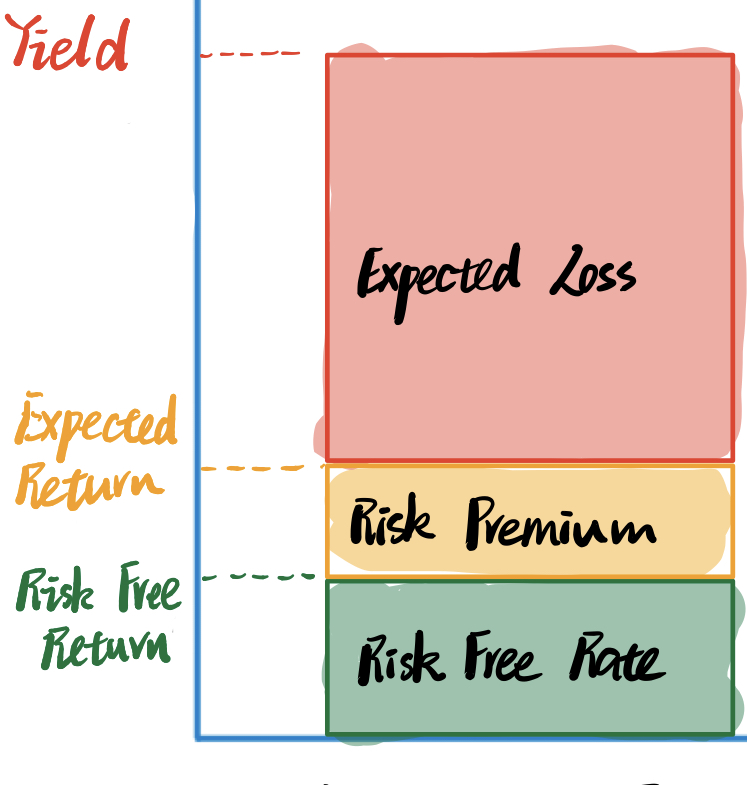
\includegraphics[width=0.1\textwidth]{yield-expected_return-risk_free_return}
        \item risk \& return in asset classes:\\
            stock $\rightarrow$ junk bond / high yield bond $\rightarrow$ investment grade bond $\rightarrow$ treasury
    \end{itemize}

    



	\end{multicols}





\newpage
    \begin{center}
         \Large{\textbf{Portfolio Choice - combine bond with stock}} \\
    \end{center}

    \begin{multicols}{2}
	\setlength{\premulticols}{1pt}
	\setlength{\postmulticols}{1pt}
	\setlength{\multicolsep}{1pt}
	\setlength{\columnsep}{2pt}

    \section{Equity Valuation}
    \begin{itemize}
        \item The concept of {\color{red}Equity}: residual claim of a firm's cash flow (received after debt payout)
        \item CAPM model: $k = r_f +\beta(r-r_f)$ 
        \item Stock Prices vs. Values \\
        	$
            \begin{cases}
                \text{1. PRICES may differ from fundamental VALUES}\\
                \text{2. Eventually, we expect convergence $P_n = V_n$}& \text{(market becomes efficient in n years)}\\
                \text{}& \text{(basis for value investing)}\\
                \text{3. If investor don't sell the stock} & \displaystyle V_0=\frac{D_0(1+g)}{k-g} \rightarrow \displaystyle P_0=\frac{D_0(1+g)}{E(r)-g}\\
                \text{we are taking the price for now}\\
                \text{see what E[r] it gives us}\\
                \rightarrow \text{Expected return = divs yield + growth in divs} & \displaystyle E(r)=\frac{D_0(1+g)}{P_0}+g\\
                \text{Things change when switch investment horizon}
            \end{cases}
            $
        \item Alternative method for long-run (LR) expected return: Profitability and Growth\\
            This is good for company with stable ROE but not stable dividend\\
            $
            \begin{cases}
                \text{When deriving the E(r) for long run: earnings yield (E/P) instead of dividend yield (D/P)}\\
                \text{Sustainable LR payout: growth = (1 – payout) $\times$ ROE }\\
            \end{cases}
            $
    \end{itemize}

    \section{Dividend Discount Model (DDM)}
    \begin{itemize}
        \item Basic Idea : Value (V) equals PV of dividends\\
        	$
            \begin{cases}
                \text{Forecast cash flows}\\
                \text{Apply discount rate (k) to cash flows}\\
            \end{cases}
            $
        \item One-stage DDM - required return on equity (k) is constant\\
        	$
            \begin{cases}
                \text{stock value from future dividend}& \displaystyle V_0=\frac{D_1}{1+k}+\frac{D_2}{(1+k)^2}+\ldots+\frac{D_n}{(1+k)^n}\\
                \text{\color{red}the difference of the 2 equations}& \text{\color{red}one is $D_1$ and one is $D_0$}\\
                \text{Dividend grows at constant rate}& \displaystyle V_0=\frac{D_0(1+g)}{1+k}+\frac{D_0(1+g)^2}{(1+k)^2}+\ldots+\frac{D_0(1+g)^n}{(1+k)^n}\\
                \text{} & \displaystyle V_0=\frac{D_0(1+g)}{k-g}\\
            \end{cases}
            $
        \item The Multi-stage DDM: - allows for multiple growth regimes\\
        	1. Economic Stimulus Could Produce Short-run Growth ‘Sugar High’\\
        	2. Valuing temporarily higher (lower) growth is similar to valuing an increase (decrease) in the initial dividend (D0)    
    \end{itemize}


    \section{Valuation multiples}
    \begin{itemize}
        \item Advantage of multiples: Avoid directly predicting cash flows and their growth 
        \item Disadvantages of multiples:\\
        	$
            \begin{cases}
                \text{Incomparable k, g, and payout of comparable stocks }\\
                \text{Inability to identify pricing inefficiencies of comparables}\\
                \text{Inconsistencies across different multiples (P/E, P/B, P/S, etc.)}\\
                \text{Instability of multiples over time}\\
            \end{cases}
            $
        \item Assumption within:\\
        	$
            \begin{cases}
                \text{Comparable assets have the same risk, CF growth, and payout as asset being valued }\\
                \text{Market pricing of comparables is efficient}\\
            \end{cases}
            $
        \item Dividend discount model (DDM) helps explain multiples (i.e., prices)\\
        	g: Stock is relatively expensive because its CFs are growing faster (higher g) than similar stocks \\
        	k: Stock is relatively expensive because its CFs are less risky (lower k, required return) than similar stocks 
        \item Interpret P/E with the DDM\\
            $
            \begin{cases}
                \text{1. P/E is price to earnings, and Dividend = Earning $\times$ Payout}\\
                \text{2. since the DDM gives us } \displaystyle V_0=\frac{D_0(1+g)}{k-g} \text{we replace dividend and divide each side with $E_0$}\\
                \text{}\displaystyle \frac{V_0}{E_0}=\frac{Payout(1+g)}{k-g}  \text{ , similarly, earning yield E/P is }\frac{E_0}{V_0}=\frac{k-g}{Payout(1+g)}\\
                \text{Interpretation 1: Stocks can have high price to earnings (P/E) ratios because g is high}\\
                \text{Interpretation 2: Stocks can have high P/E because discount rate (k) is low}\\
                \text{Wee need to determine which factor it is that lead to a high P/E !!!}\\
            \end{cases}
            $
    \end{itemize}

    \section{Portfolio Optimization}
    \begin{itemize}
        \item We move from long-term return to short-term return\\
            $
            \begin{cases}
                \text{For long-term holding valuation: }\displaystyle E(r)=\frac{D_0(1+g)}{P_0}+g\\
                \text{}\\
                \text{For short-term holding valuation: }\displaystyle E(r_1)=\frac{V_0(1+k)}{P_0}-1\\
            \end{cases}
            $
        \item Sharp Ratio: the risk premium per unit of risk: $\displaystyle SR_{us} = \frac{E[r_{us}]-f_f}{\sigma_{us}}$\\
            (As an investor, we always want a high sharp ratio, that's the essense of MVE)
        \item Mean Variance Efficient MVE: Diversification help us increase the sharp ratio\\
            (In other words, MVE is the portfolio with the highest sharp ratio)\\
            (We achieve it by adjusting the weights in different asset, and see the final outcome)
        \item Mean-Variance Utility: $U_p = E(r_p) - \frac{1}{2}A(\sigma_p)^2$ , with ``A'' being the risk aversion
        \item Optimal Portfolio Weights (weights in risky asset): $w_{MVE}^* = \frac{E[r_{MVE}]-r_f}{A\sigma_{MVE}^2}$
    \end{itemize}

    \section{Applying the CAPM}
    \begin{itemize}
        \item CAPM: build on the idea that everyone holds the unique best portfolio.\\
            That is the market portfolio: $SR_p \leq SR_m = \frac{E[r_M]-r_f}{\sigma_m}$
        \item Market portfolio: all risky assets held in proportion to their market capitalization
        \item For each asset: the weights should equate teh marginal reward-risk ratios\\
            $\displaystyle E[r_i]-r_f = \beta_{i,MVE} \times (E[r_{MVE}] - r_f)$\\
            (if one asset is ``x'' times riskier than the market, we require ``x'' times excess return)
        \item Market Risk Premium: $\displaystyle w_{M}^* = \frac{E[r_m]-r_f}{A\sigma_m^2} \longrightarrow {\color{red}E[r_m]-r_f} = w_m^*A\sigma_m^2$\\
            If keep weights in market same, then a rise in A or $\sigma_m$ ask for higher market risk premium\\
            If keep the same expectation in market risk premium, a change in A or $\sigma_m$ changes weights
        \item SML: Security Market Line
            $
            \begin{cases}
                E\left[r_{i}\right]-r_{f}=\beta_{i}\left(E\left[r_{M}\right]-r_{f}\right) \text{ with } \displaystyle \beta_{i}=\frac{\rho_{i, M} \sigma_{i}}{\sigma_{M}}=\frac{\operatorname{Cov}\left(r_{i}, r_{M}\right)}{\sigma_{M}^{2}}\\
                {\color{red}E\left[r_{i}\right]=r_{f}+\beta_{i}\left(E\left[r_{M}\right]-r_{f}\right)}\\
                \text{shows how required returns depend on risk }\beta\\
                \text{Required and expected returns are the same in efficient markets}\\
            \end{cases}
            $
        \item $\alpha$ = expcected return - CAPM required return. A "mispriced" stock has $\alpha \neq 0$
        \item SCL: Security Characteristic Line: {\color{red}$r_{i t}-r_{f t}=\alpha_{i}+\beta_{i}\left(r_{m t}-r_{f t}\right)+e_{i t}$}\\
            $ \underbrace{\sigma_{i}^{2}}_{\text{total variance / risk}}= 
            \underbrace{\beta_{i}^{2} \sigma_{M}^{2}}_{\text{Systematic risk}}+
            \underbrace{\sigma_{e_{i}}^{2}}_{\text{Idiosyncratic risk}}$\\
            Systematic risks contribute to the overall risk of any portfolio.\\
            Idiosyncratic risks can be diversified away in a portfolio\\
            The SCL regression R2 is (systematic risk)/(total risk) $\displaystyle R^{2}=\frac{\beta_{i}^{2} \sigma_{M}^{2}}{\sigma_{i}^{2}}$
            % $
            % \begin{cases}
            %     \text{}\\
            %     \text{}\\
            %     \text{}\\
            %     \text{}\\
            % \end{cases}
            % $
    \end{itemize}

    \section{CAPM Anomalies}
    \begin{itemize}
        \item Anomalies $\rightarrow$ alpha:
            $
            \begin{cases}
                \text{Size (market capitalizaion): small beats big, but this effect is eaker recently}\\
                \text{Value (B/M): high book to market ratio beats the growth}\\
                \text{Beta: low beta beats high bta in risk-adjusted return (alpha)}\\
                \text{Momentum: Past winner perform bad in the future}\\
            \end{cases}
            $
        \item How to quantify the effect:
            $
            \begin{cases}
                \text{SMB: real excess return - theoretical return}\\
                \text{HML (value premium): retur of high B/M - return of low B/M}\\
                \text{Beta: }\\
                \text{UMD Momentum: up stock - down stocks}
            \end{cases}
            $
        \item The Fama and French Three-Factor Model:\\
            {\color{red}$r_{i t}-r_{f_{t}}=\alpha_{i}^{\mathrm{FF} 3}+\beta_{i}\left(r_{m t}-r_{f_{t}}\right)+s_{i} S M B_{t}+h_{i} H M L_{t}+e_{i t}$}\\
            $
            \begin{cases}
                \text{Market Factor: } MktRf_t = r_{mt} - r_{ft}\\
                \text{HML (value premium): retur of high B/M - return of low B/M}\\
                \text{Beta: }\\
                \text{Momentum Factor: } UMD_{t}=r_{Ut}-r_{Dt}  \\
            \end{cases}
            $\\
            {\color{red}$\underbrace{r_{i t}-r_{f_{t}}}_{\text{asset excess return} }=\alpha_{i}^{\mathrm{FF} 3}+\beta_{i}\left(r_{m t}-r_{f_{t}}\right)+s_{i} S M B_{t}+h_{i} H M L_{t}+e_{i t}$}\\
            Coefficients $s_{i}$ and $h_{i}$ are size and value betas (loadings)\\
            Small (big) firms usually have positive (negative) $s_{i}$ values \\
            Value (growth) firms usually'have positive (negative) $h_{i}$ values
        \item Information Ratio:\\
            Meaning: extra return we can obtain from analysis, compare to, \\
            Scenario: For an investor holding the market, how much will Sharpe ratio improve if optimally weights BRK?\\
                $S R_{N e w}=\sqrt{SR_{Init}^{2}+IR^{2}}$\\
                $S R_{\text {Portfolio }}^{2}=S R_{\text {Market }}^{2}+\left[\displaystyle \frac{\alpha_{A}}{\sigma\left(e_{A}\right)}\right]^{2}$
    \end{itemize}

    \section{Performance evaluation: skill vs luck}
    \begin{itemize}
        \item The CAPM and multifactor models allow us to analyze average returns, risk, and investment strategies:\\
            $
            \begin{cases}
                \text{Average returns: How much is alpha and how much is beta?}\\
                \text{Risk: How much is systematic and how much is idiosyncratic?}\\
                \text{Strategies: Are we using value/growth or small/big, etc.?}\\
            \end{cases}
            $
        \item actively managed funds: managers pick the portfolio weights\\
            Example: ClearBridge Large Cap Growth Fund (Legg Mason)
            $
            \begin{cases}
                \text{people manage the fund}\\
                \text{Sold by advisers and brokers}\\
                \text{large-cap growth stocks}\\
                \text{Annual turnover (trading) 20\%}\\
            \end{cases}
            $
        \item passively managed index funds: computers pick index weights\\
            Example: Vanguard 500 Index Fund (Vanguard)
            $
            \begin{cases}
                \text{umans program computer to manage}\\
                \text{track performance of S\&P500 Index}\\
                \text{Directly sold to investors}\\
                \text{Annual turnover (trading) 4\%}\\
            \end{cases}
            $\\
            Usually, index fund with the lowest expense ratio have higher return\\
            \begin{tabular}{|lcr|}
            \hline Ticker & Expense Ratio & $2000-2015$ Avg. Return \\
            \hline AAFPX & $0.60 \%$ & $4.71 \%$ \\
            PREIX & $0.34 \%$ & $5.01 \%$ \\
            VFINX & $0.17 \%$ & $5.16 \%$ \\
            SPY & $0.09 \%$ & $5.19 \%$ \\
            \hline
            \end{tabular}
        \item Open-ended mutual funds
            $
            \begin{cases}
                \text{don’t trade on the open market}\\
                \text{executed at net asset value (NAV) at end of day market close}\\
                \text{can’t watch price fluctuate minute by minute like a stock}\\
                \text{repriced based on number of shares bought and sold}\\
            \end{cases}
            $
        \item Exchange-traded Funds
            $
            \begin{cases}
                \text{}\\
                \text{}\\
                \text{}\\
                \text{}\\
            \end{cases}
            $
        \item Closed End Funds
            $
            \begin{cases}
                \text{Similar to ETFs but actively managed}\\
                \text{CEFs launch through an IPO, only set amt of shares enter market}\\
                \text{supply and demand determining price}\\
                \text{CEFs higher fees}\\
            \end{cases}
            $
    \end{itemize}


            % $
            % \begin{cases}
            %     \text{}\\
            %     \text{}\\
            %     \text{}\\
            %     \text{}\\
            % \end{cases}
            % $

    \end{multicols}















% \newpage
%     \begin{center}
%          \Large{\textbf{Why investment with machine learning is so hard}} \\
%     \end{center}


%     \section{}
%     \begin{itemize}
%         \item 
%         \item 
%         \item 
%         \item 
%         \item 
%         \item 
%         \item 
%     \end{itemize}


%             $
%             \begin{cases}
%                 \text{}\\
%                 \text{}\\
%                 \text{}\\
%                 \text{}\\
%             \end{cases}
%             $






































\newpage



\begin{center}
     \Large{\textbf{Quantitative Finance -- Derivatives}} \\
\end{center}

\begin{multicols}{2}
\setlength{\premulticols}{1pt}
\setlength{\postmulticols}{1pt}
\setlength{\multicolsep}{1pt}
\setlength{\columnsep}{2pt}


\section{Time value of money}
\begin{itemize}
	\item money has time value, because we can reinvest them
	\item always picture a timeline in thinking about this problem
\end{itemize}

\section{Interest}
\begin{itemize}
	\item The easiest way to make money is by earning interest from the bank
	\item simple interest rate (return calculation): $a_t = a_0*(1+it)$
	\item compound interest rate (keep reinvest): $a_t = a_0(1+i)^t$
	\item effective interest rate during a period: $i = \frac{a_n - a_{n-1}}{a_{n-1}}$
	\item nominal rate of interest: $i^{(m)}$, meaning that this interest i is paid m times a year\\
		an amount of $\frac{i^{(m)}}{m}$ will be paid at each time interval, therefore at the end $=(1+\frac{i^{(m)}}{m} )^m$\\
		let m goes to infinity, we have the continuous form $(1+\frac{r}{m} )^{mt} \longrightarrow e^{rt}$
	
\end{itemize}

\section{Annuities and Perpetuities}
\begin{itemize}
	\item annuity: fixed payment at each time point\\
			annuity-immediate: payment at the end of interval\\
			annuity-due: payment at the beginning of interval
	\item perpetuities: fixed payment at each time point, until infinity\\
		perpetuity-immediate: payment at the end of interval\\
		perpetuity-due: payment at the beginning of interval
\end{itemize}

\section{Bonds: a fixed income instrument}
\begin{itemize}
	\item market graph of bonds: what kinds of bonds are out there
	\item zero coupon bond: no coupon payment, only pay face value at maturity (treat as discount)\\
			zero rate: the annualized rate of return (annual compound) $\longrightarrow B(t,T)(1+R(t,T))^{T-t} = 1$\\
			continuous zero rate: $\longrightarrow B(t,T)e^{(T-t)R(t,T)} = 1$   [treat R(t,T) as an interest rate]\\
			k-times per year: $\longrightarrow B_{(t,T)}(1+\frac{R_{(r,T)}}{m} )^m(T-t) = 1$
	\item Bond with coupon: pay at specific time\\
			
			Yield-to-Maturity: the interest rate that makes present value of cash flow equals bond price\\
			or we can say that the YTM is the IRR at this point: internal rate of return\\
			it tells us the interest rate that this investment is representing, so that we can compare\\
			
			Annual Coupon Bond: $P = \sum \frac{CF_t}{(1+y)^t}$\\
			Semi annual coupon bond: $P = \sum \frac{CF_t}{(1+\frac{y}{2	} )^{2t}}$\\
			
			So what happened in the market $\longrightarrow$ we calculate the bond price, by the risk-free rate\\
			Therefore it is easy to imagine: \\
			if risk-free rate goes up, the current bond price should drop\\
			if risk-free rate goes down, the current bond price should rise\\
			In short, the bond price is negatively correlated to the YTM\\
			
			It depends on how we structure the dependent variable and independent variables:\\
			1. Calculate the bond price: the DV is bond price, IDV is the interest rate, negative correlated.\\
			2, Calculate YTM: the DV is YTM, IDV is bond price, if bond price is high, meaning the YTM must be low\\
	\item Relationship between zero coupon bond and coupon bond:\\
			When a coupon bond pays no coupon, it is the same as zero coupon bond $\longrightarrow$ same price and YTM\\
			With coupon bond introduce coupon, we have 2 dimension to interpret the results:\\
			1. how the price will change: with introduction of future cash flow, interest rate does not change, price will rise; with price rise, the YTM will drop\\
			2. how the YTM will change: not a good direction, stick to PRICE $\longrightarrow$ YTM path
	\item Since the zero coupon bond has a higher YTM than coupon bond, it is some how confusing because we may think the coupon bond gives us more return.
	\item We introduce the "Par Yield" to do standardization on the returns:\\
	\item	Par Bond: the price = face value $\longrightarrow$ issue at par $\longrightarrow$ YTM = annual coupon rate\\
		Par Yield: when a bond is issue at par, the coupon rate (annualized return) is equal to YTM (calculated annualized return)
	\item Dollar Duration: the $\frac{dP}{dy}$ the derivatives of price w.r.t. YTM\\
			Modified Duration: $-\frac{1}{P} \frac{dp}{dy}$, Dur normalized by price\\
			Dollar Value of 1 basis point (DV01): $ = Dur \cdot (-1 bp)$\\
			
			At a specific price level, the Dollar Duration Dur, decrease as:\\
			1. maturity increase (Dur is a price sensitivity measure to yield, with T goes up, it is more sensitive)\\
			2. coupon increases (1. more money to discount, more sensitive. 2. more coupon means price up, then more sensitive)\\
			3. YTM decrease (look at the graph, when YTM is small, it is steeper)\\
	
\end{itemize}

\section{Forward Rates}
\begin{itemize}
	\item Diagram and calculation: separate the time into different intervals, make investment using respective rates
	\item 
\end{itemize}


\section{Futures}


\section{Options}
* Memoryless:\\

\section{Bonds}
* Memoryless:

\end{multicols}





% -----------------------------------------------------------------------
% -----------------------------------------------------------------------
% -----------------------------------------------------------------------





\newpage

%\includegraphics[width=60mm,scale=1]{images/PACF-2.png}
\begin{center}
     \Large{\textbf{Financial Assets: Derivatives}} \\
\end{center}

\begin{multicols}{2}
\setlength{\premulticols}{1pt}
\setlength{\postmulticols}{1pt}
\setlength{\multicolsep}{1pt}
\setlength{\columnsep}{2pt}


\section{Forwards / Futures}
\begin{itemize}
	\item Futures: Traded in the exchange, so basically standardized contract
	\item Forwards: customized
	\item Keywords: strike price, maturity day, long, short\\
	
	Agencies
	\item Clearing house: ensure trader fulfill obligations
	\item Margin: Trader deposit margin to fulfill obligations:\\
		Initial margin ; Maintenance margin ; Variation margin ;
	\item 
	
\end{itemize}

\section{Options}
\begin{itemize}
	\item Vanilla Option / European Option: fixed maturity date, strike price
	\item American Option: can exercise before maturity date
	\item Bermudan Option: can exercise on pre-determined date
	\item Barrier Option: can exercise once cross the barrier level: \\
			up and out, down and out, up and in, down and in\\
			1) Callable Bull: if always bull, then it is valid (never drop down barrier) [down and out]
			2) Callable Bear: if always bear, then it is valid (never go up barrier) [up and out]
			
	\item Asian Option: the payoff determined by average price of pre-set period of time\\
	
	Option strategies: Notice difference between prices and payoff
	\item Straddle: long 1 call and 1 put with same K and T
	\item Strangle: long call and put with same K and T
	\item Bull Spread: make money when price up: Buy call with $K_1$, sell call with $K_2$
	\item Bear Spread: make money when price down: Buy call with $K_1$, sell call with $K_2$
	\item Butterfly: long 2 calls, short call * 2
	
\end{itemize}

\section{Warrents}
\begin{itemize}
	\item equity warrants: issue by company. represent the right to subscribe to equity securities
	\item derivative warrants: issued by 3rd party.
\end{itemize}

\section{Swap: 2 parties exchange financial instruments}
\begin{itemize}
	\item Interest rate swap\\
			A: expect Libor drops ; B: expect Libor ups\\
			????
	\item Benefit: 1) hedge against interest rate exposure ; 2) leverage comparative advantage\\
			A: AAA rated company ; B: BBB rated company.\\
			Company A will definitely have less lending interest rate in the market, in all loans\\
			But that doesn't mean company A can't do better. We can calculate the spread and see what is company A's comparative advantage, and borrow only that kind of loan, other company can use their comparative advantage P38
	\item 
\end{itemize}


\end{multicols}





% -----------------------------------------------------------------------
% -----------------------------------------------------------------------
% -----------------------------------------------------------------------


\newpage

\begin{center}
     \Large{\textbf{Financial Risk: Value at Risk}} \\
\end{center}

\begin{multicols}{2}
\setlength{\premulticols}{1pt}
\setlength{\postmulticols}{1pt}
\setlength{\multicolsep}{1pt}
\setlength{\columnsep}{2pt}

\section{Return}
\begin{itemize}
	\item Arithmetic Return: $R_t = \frac{S_t - S_{t-1}}{S_{t-1}}$
	\item Log Return: $log(1+R_t) = log(\frac{S_t}{S_{t-1}}) = log(S_t) - log(S_{t-1})$
\end{itemize}

\section{Volatility Measure}
\begin{itemize}
	\item $\sigma_s = \sqrt{\frac{1}{n-1} \sum (\mu_i - \bar \mu)^2}$
	\item Then the volatility over N periods: $\sqrt{N}\sigma_s$
\end{itemize}

\section{VaR: Value-at-Risk}
\begin{itemize}
	\item if there is a distribution graph, starting from left to some point, this region is $\alpha$
	\item the rest region to the right is $1-\alpha$, stands for the confidence: 95\%, 99\% etc.
	\item We called $\alpha$ as the "tail probability", since it is the worst scenario
	\item In a graphical sense, VaR is the $p-th$ quantile of the PnL distribution
	\item "Relative VaR": $E[PnL] - VaR$
\end{itemize}

\section{Modeling the PnL distribution}
\begin{itemize}
	\item The fundamental of finding VaR is to model the portfolio PnL distribution
	\item Parametric Approach:\\
			Keypoint: construct the mean $\mu$ and volatility $\sigma$\\
			Approach: convert to approach "standard normal distribution"\\
			Then we can calculate VaR ; or extend this to a multi-time period scenario\\
	\item Non-Parametric Approach: Historical Simulation\\
			1. we want to know the price at tomorrow\\
			2. we convert the a problem: how much will the portfolio value change\\
			3. based on past period-wise change data, we treat it as distribution\\
			4. select the change we need\\
\end{itemize}
			
\end{multicols}


\begin{center}
     \Large{\textbf{Financial Risk: Hedging, Optimal Hedging}} \\
\end{center}

\begin{multicols}{2}
\setlength{\premulticols}{1pt}
\setlength{\postmulticols}{1pt}
\setlength{\multicolsep}{1pt}
\setlength{\columnsep}{2pt}

\section{Idea}
\begin{itemize}
	\item Hedge against a instrument that is negatively correlated to your portfolio
\end{itemize}

\section{Quantify}
\begin{itemize}
	\item we want to minimize variance of new portfolio : $S+NF$, with $S$ original portfolio
	\item we first construct the variance: $\sigma_s + N^2 \sigma_f + 2N\sigma_{s,f}$
	\item Then N can be solved by using the solution for a square equation
\end{itemize}

\end{multicols}

% -----------------------------------------------------------------------
% -----------------------------------------------------------------------
% -----------------------------------------------------------------------





\newpage

\begin{center}
     \Large{\textbf{Coursera - Columbia - No Arbitrage}} \\
\end{center}

\begin{multicols}{2}
\setlength{\premulticols}{1pt}
\setlength{\postmulticols}{1pt}
\setlength{\multicolsep}{1pt}
\setlength{\columnsep}{2pt}

\section{Example of using No-Arbitrage pricing: }
\begin{itemize}
	\item \text{\color{red}1. A bond that pays A in 1 year:}
		\\Pricing 1: portfolio that: buy 1 bond, borrow $\frac{A}{1+r}$
		\\Pricing 2: portfolio that: sell 1 bond, lend $\frac{A}{1+r}$
	\item \text{\color{red}2. Use compounding interest rate for pricing:}
	\item \text{\color{red}3. Floating Rate Bond:}
		\\The price of a floating rate bond, is equal to, the face value.
	\item 
\end{itemize}


			
\end{multicols}


\begin{center}
     \Large{\textbf{Cousera - Columbia - No Arbitrage in various assets}} \\
\end{center}

\begin{multicols}{2}
\setlength{\premulticols}{1pt}
\setlength{\postmulticols}{1pt}
\setlength{\multicolsep}{1pt}
\setlength{\columnsep}{2pt}

\section{Swaps}
\begin{itemize}
	\item What is it: a trade between fixed and float rates
	\item Why is it: leverage relative strength, capture trends in other markets
	\item How does it works: do your best, borrow your weakness
		\\1. A has relative strength in fixed rate
		\\2. B has relative strength in floating rate
		\\3. A will borrow fixed rate, B will borrow floating rate
		\\4. A borrow floating from B, pays fixed to B 
	\item How to price it: What should be the exchange rate pay to each other
		\\1. Swap should be of 0 value to each party
		\\2. Write the Cash Flow PV for one side
		\\3. Set it to 0 and we calculate the payment rate
\end{itemize}

\section{Futures}
\begin{itemize}
	\item What is it: An traded an exchange standardized contract
	\item Why need it: standardized, counter party risk, solved multiple price for same maturity
	\item How does it works: Margin call (go to initial margin), clearing house
	\item How to price it: 
		\\
	\item Minimum variance hedging (since perfect hedge is impossible):
		\\
\end{itemize}

\section{Options}
\begin{itemize}
	\item In the money, at the money, out of the money
	\item Put-Call Parity: call + cash = put + stock
		\\ try to buy a stock, and use money to help me
		\\ try to sell a stock, and hold a stock to help me
		\\ $C + Ke^{-rt} = P + S$
		\\ $C + Ke^{-rt} = P + S - D$ (with dividend)
	\item Bounds of option prices
\end{itemize}

\section{Binomial Tree Pricing}
\begin{itemize}
	\item 1-period Binomial Tree: price goes up and down with probabilities, allow short sell
	\item Multi-period Binomial Tree: extend with same prob and up/down scale
	\item Replications: (buying shares, investing in cash) $\leftrightarrow$ (option)
		\\ make the payoff equals
	\item European and American Pricing: use risk-neutral prob to price:
		\\ $q = \frac{R-d}{u-d}$. $C_0 = \frac{1}{R} [qC_u + (1-q)C_d ]$
\end{itemize}


\end{multicols}

% -----------------------------------------------------------------------
% -----------------------------------------------------------------------
% -----------------------------------------------------------------------










% style end
% -----------------------------------------------------------------------
\end{document}
% -----------------------------------------------------------------------
